\documentclass[]{article}
\usepackage{lmodern}
\usepackage{amssymb,amsmath}
\usepackage{ifxetex,ifluatex}
\usepackage{fixltx2e} % provides \textsubscript
\ifnum 0\ifxetex 1\fi\ifluatex 1\fi=0 % if pdftex
  \usepackage[T1]{fontenc}
  \usepackage[utf8]{inputenc}
\else % if luatex or xelatex
  \ifxetex
    \usepackage{mathspec}
  \else
    \usepackage{fontspec}
  \fi
  \defaultfontfeatures{Ligatures=TeX,Scale=MatchLowercase}
  \newcommand{\euro}{€}
    \setmainfont[]{DejaVu Sans}
\fi
% use upquote if available, for straight quotes in verbatim environments
\IfFileExists{upquote.sty}{\usepackage{upquote}}{}
% use microtype if available
\IfFileExists{microtype.sty}{%
\usepackage{microtype}
\UseMicrotypeSet[protrusion]{basicmath} % disable protrusion for tt fonts
}{}
\usepackage[margin=1in]{geometry}
\usepackage{hyperref}
\PassOptionsToPackage{usenames,dvipsnames}{color} % color is loaded by hyperref
\hypersetup{unicode=true,
            pdftitle={2\_Respondents\_Profiling},
            pdfborder={0 0 0},
            breaklinks=true}
\urlstyle{same}  % don't use monospace font for urls
\usepackage{color}
\usepackage{fancyvrb}
\newcommand{\VerbBar}{|}
\newcommand{\VERB}{\Verb[commandchars=\\\{\}]}
\DefineVerbatimEnvironment{Highlighting}{Verbatim}{commandchars=\\\{\}}
% Add ',fontsize=\small' for more characters per line
\usepackage{framed}
\definecolor{shadecolor}{RGB}{248,248,248}
\newenvironment{Shaded}{\begin{snugshade}}{\end{snugshade}}
\newcommand{\KeywordTok}[1]{\textcolor[rgb]{0.13,0.29,0.53}{\textbf{{#1}}}}
\newcommand{\DataTypeTok}[1]{\textcolor[rgb]{0.13,0.29,0.53}{{#1}}}
\newcommand{\DecValTok}[1]{\textcolor[rgb]{0.00,0.00,0.81}{{#1}}}
\newcommand{\BaseNTok}[1]{\textcolor[rgb]{0.00,0.00,0.81}{{#1}}}
\newcommand{\FloatTok}[1]{\textcolor[rgb]{0.00,0.00,0.81}{{#1}}}
\newcommand{\ConstantTok}[1]{\textcolor[rgb]{0.00,0.00,0.00}{{#1}}}
\newcommand{\CharTok}[1]{\textcolor[rgb]{0.31,0.60,0.02}{{#1}}}
\newcommand{\SpecialCharTok}[1]{\textcolor[rgb]{0.00,0.00,0.00}{{#1}}}
\newcommand{\StringTok}[1]{\textcolor[rgb]{0.31,0.60,0.02}{{#1}}}
\newcommand{\VerbatimStringTok}[1]{\textcolor[rgb]{0.31,0.60,0.02}{{#1}}}
\newcommand{\SpecialStringTok}[1]{\textcolor[rgb]{0.31,0.60,0.02}{{#1}}}
\newcommand{\ImportTok}[1]{{#1}}
\newcommand{\CommentTok}[1]{\textcolor[rgb]{0.56,0.35,0.01}{\textit{{#1}}}}
\newcommand{\DocumentationTok}[1]{\textcolor[rgb]{0.56,0.35,0.01}{\textbf{\textit{{#1}}}}}
\newcommand{\AnnotationTok}[1]{\textcolor[rgb]{0.56,0.35,0.01}{\textbf{\textit{{#1}}}}}
\newcommand{\CommentVarTok}[1]{\textcolor[rgb]{0.56,0.35,0.01}{\textbf{\textit{{#1}}}}}
\newcommand{\OtherTok}[1]{\textcolor[rgb]{0.56,0.35,0.01}{{#1}}}
\newcommand{\FunctionTok}[1]{\textcolor[rgb]{0.00,0.00,0.00}{{#1}}}
\newcommand{\VariableTok}[1]{\textcolor[rgb]{0.00,0.00,0.00}{{#1}}}
\newcommand{\ControlFlowTok}[1]{\textcolor[rgb]{0.13,0.29,0.53}{\textbf{{#1}}}}
\newcommand{\OperatorTok}[1]{\textcolor[rgb]{0.81,0.36,0.00}{\textbf{{#1}}}}
\newcommand{\BuiltInTok}[1]{{#1}}
\newcommand{\ExtensionTok}[1]{{#1}}
\newcommand{\PreprocessorTok}[1]{\textcolor[rgb]{0.56,0.35,0.01}{\textit{{#1}}}}
\newcommand{\AttributeTok}[1]{\textcolor[rgb]{0.77,0.63,0.00}{{#1}}}
\newcommand{\RegionMarkerTok}[1]{{#1}}
\newcommand{\InformationTok}[1]{\textcolor[rgb]{0.56,0.35,0.01}{\textbf{\textit{{#1}}}}}
\newcommand{\WarningTok}[1]{\textcolor[rgb]{0.56,0.35,0.01}{\textbf{\textit{{#1}}}}}
\newcommand{\AlertTok}[1]{\textcolor[rgb]{0.94,0.16,0.16}{{#1}}}
\newcommand{\ErrorTok}[1]{\textcolor[rgb]{0.64,0.00,0.00}{\textbf{{#1}}}}
\newcommand{\NormalTok}[1]{{#1}}
\usepackage{graphicx,grffile}
\makeatletter
\def\maxwidth{\ifdim\Gin@nat@width>\linewidth\linewidth\else\Gin@nat@width\fi}
\def\maxheight{\ifdim\Gin@nat@height>\textheight\textheight\else\Gin@nat@height\fi}
\makeatother
% Scale images if necessary, so that they will not overflow the page
% margins by default, and it is still possible to overwrite the defaults
% using explicit options in \includegraphics[width, height, ...]{}
\setkeys{Gin}{width=\maxwidth,height=\maxheight,keepaspectratio}
\setlength{\parindent}{0pt}
\setlength{\parskip}{6pt plus 2pt minus 1pt}
\setlength{\emergencystretch}{3em}  % prevent overfull lines
\providecommand{\tightlist}{%
  \setlength{\itemsep}{0pt}\setlength{\parskip}{0pt}}
\setcounter{secnumdepth}{0}

%%% Use protect on footnotes to avoid problems with footnotes in titles
\let\rmarkdownfootnote\footnote%
\def\footnote{\protect\rmarkdownfootnote}

%%% Change title format to be more compact
\usepackage{titling}

% Create subtitle command for use in maketitle
\newcommand{\subtitle}[1]{
  \posttitle{
    \begin{center}\large#1\end{center}
    }
}

\setlength{\droptitle}{-2em}
  \title{2\_Respondents\_Profiling}
  \pretitle{\vspace{\droptitle}\centering\huge}
  \posttitle{\par}
  \author{}
  \preauthor{}\postauthor{}
  \date{}
  \predate{}\postdate{}


% Redefines (sub)paragraphs to behave more like sections
\ifx\paragraph\undefined\else
\let\oldparagraph\paragraph
\renewcommand{\paragraph}[1]{\oldparagraph{#1}\mbox{}}
\fi
\ifx\subparagraph\undefined\else
\let\oldsubparagraph\subparagraph
\renewcommand{\subparagraph}[1]{\oldsubparagraph{#1}\mbox{}}
\fi

\usepackage{booktabs}
\usepackage{longtable}
\usepackage{array}
\usepackage{multirow}
\usepackage[table]{xcolor}
\usepackage{wrapfig}
\usepackage{float}
\usepackage{colortbl}
\usepackage{pdflscape}
\usepackage{tabu}
\usepackage{threeparttable}
\usepackage{threeparttablex}
\usepackage[normalem]{ulem}
\usepackage{makecell}

\begin{document}
\maketitle

Generally, this is the variation of the software classification, though,
in the center of it respondents and instead of MDS and K-mean Latent
Profile Analysis is used. Firstly, it is convenient wrapper, secondly,
it is specifically suited for the survey kind of data. What I haven't
used yet, though, might be useful is fixed/freed/random means across
various profiles - they might represent our expectations about the
profiles characteristic, such as mean age or typical occupation.

\emph{What else could it be used for}: in the next report I will try to
make LPA on Occupation+Education+Age and use profiles probability to map
software

Showing job shifts in connection with associated software is not
possible due to NAs in Q21\_1\_open (previous job): there is
\texttt{sum(df\_clean\$Q22\ ==\ "")} NAs, while the total complete
sample is \texttt{nrow(df\_clean)}.

TODO: what I need to do is to consider public/private sector\\
Q19 - do you work in a public/private sector

Description of items for LPA

\begin{Shaded}
\begin{Highlighting}[]
\CommentTok{# Q1 - language}

\CommentTok{# Q3_1 - Desktop}
\CommentTok{# Q3_2 - Laptop}
\CommentTok{# Q3_3 - Tablet}
\CommentTok{# Q3_4 - Mobile phone/Smartphone}
\CommentTok{#}

\CommentTok{# Q8_v2_1 - Built-in default settings}
\CommentTok{# Q8_v2_2 - Plugins/add-ons/extensions}
\CommentTok{# Q8_v2_3 - Script to extend Software}
\CommentTok{# Q8_v2_4 - I reprogram}

\CommentTok{# Traditional Surveys}
\CommentTok{# Q9 - Q10 - Q11 - Q12 - Q13 - Q14 - Q15 - Q16 - Q16}

\CommentTok{# Q17_R - employment status}
\end{Highlighting}
\end{Shaded}

Latent Profile Analysis is used in social science and educational
research. It suits the needs to aggregate reprogrammability items,
though, need to check how it will deal with Occupations and SES.

Number of profiles to choose - analytically - less BIC is better.

\begin{tabu} to \linewidth {>{\raggedright}X>{\raggedleft}X>{\raggedleft}X>{\raggedleft}X>{\raggedleft}X}
\hline
n\_profiles & Constrained variance, fixed covariance & Freed variance, fixed covariance & Constrained variance, constrained covariance & Freed variance, freed covariance\\
\hline
1 & -61164.26 & -59565.16 & -55664.78 & -55664.78\\
\hline
2 & -59305.92 & NA & -55313.01 & NA\\
\hline
3 & -58064.10 & NA & -54427.77 & NA\\
\hline
4 & -56775.90 & NA & -54683.45 & NA\\
\hline
5 & -56403.10 & NA & -54388.93 & NA\\
\hline
6 & -56230.51 & NA & -54439.99 & NA\\
\hline
\end{tabu}

Number of profiles to choose - visually.

Freed variance - variance might vary across the groups. Constrained
variance means that profiles are chosen according to the assumption that
variance should be closely the same in all of the profiles. Fixed
variance indicates the strength of this assumption, so, variance is less
then in case of Constrained Variance.

In it's turn, covariance indicate the degree of variation for
interconnection of variables across profiles. Basic example - income
should be equally connected with education across all profiles in case
of fixed covariance.

Two models are plotted:

\begin{itemize}
\tightlist
\item
  Constrained variance, fixed covariance
\item
  Constrained variance, constrained covariance (+)
\end{itemize}

Based on the BIC, we should choose EEE = Constrained variance,
constrained covariance model = model 2.

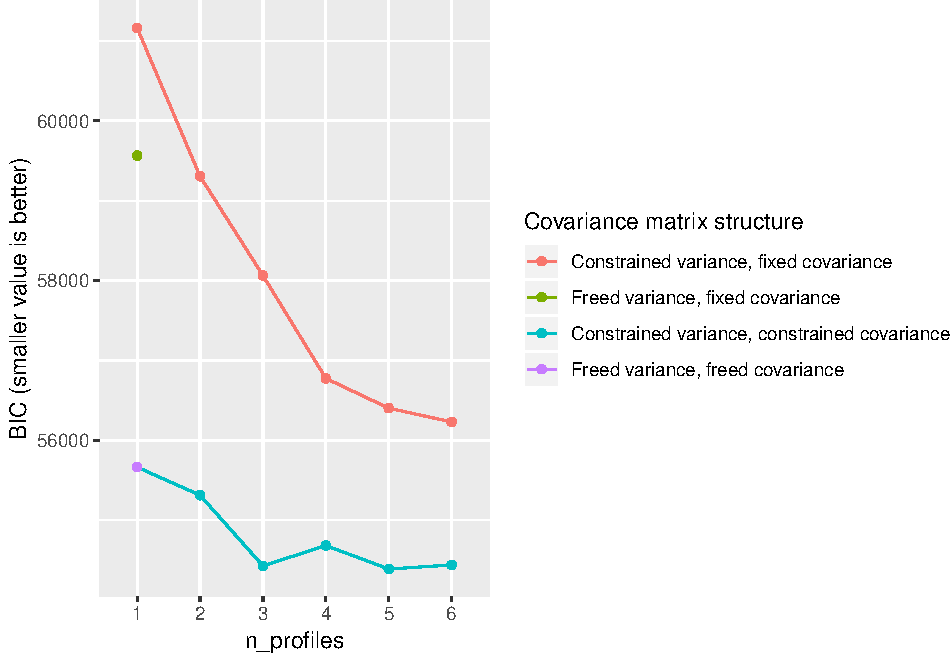
\includegraphics{/home/stlk/projects/appcentriccomp/reports/030_latent_profile_analysis_files/figure-latex/unnamed-chunk-7-1.pdf}

Choosing the model with 5 profiles.

Plotting

\begin{figure}[htbp]
\centering
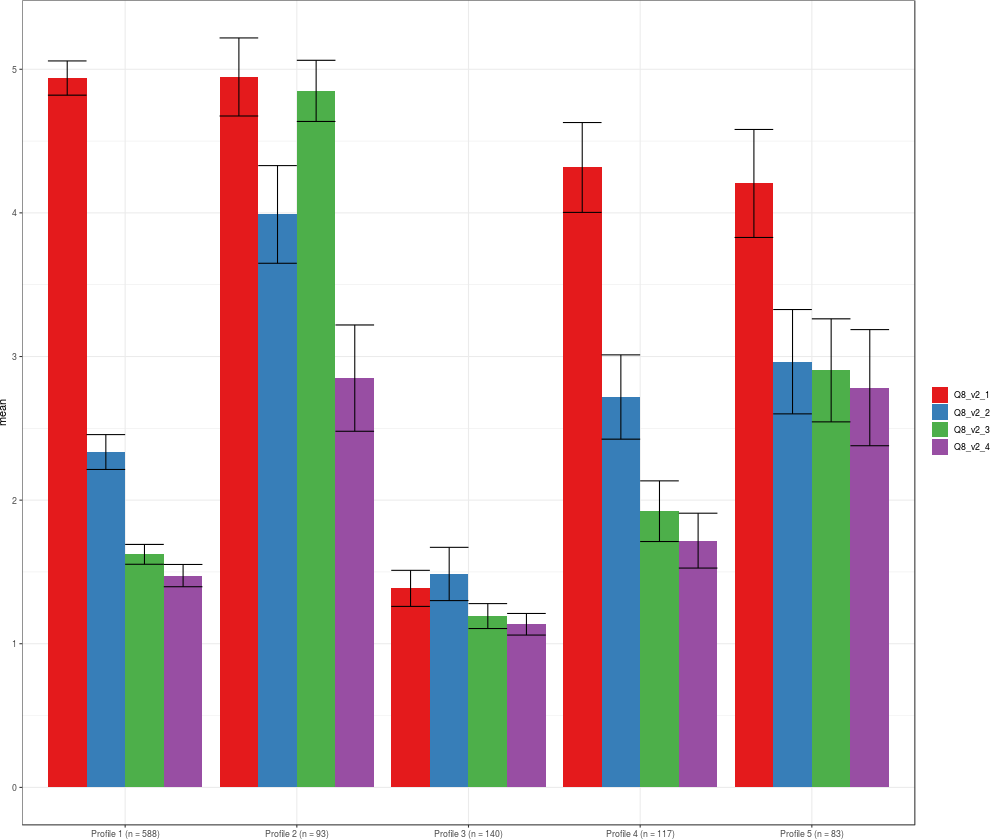
\includegraphics{/home/stlk/projects/appcentriccomp/reports/030_latent_profile_analysis_files/figure-latex/unnamed-chunk-10-1.png}
\caption{Reprogrammability Items Across Profiles: Will make a bit more
sense later in conjunction with Occupations}
\end{figure}

Here just a brief description I made in Overleaf some time ago.

Using Latent Profile Analysis 5 consistent groups of respondents were
extracted. 1st profile is the largest one (588), respondents in other
profiles are distributed more or less uniformaly.

Figure 1 demonstrates profile differences of responses about extension
or reprogrammability of software. Firstly, it should be noted that
respondents across all of the profiles tend to change built-in settings
of the software they are using. Notably, the the respondents from
\emph{1 profile} have one of the lowest dispersion on this item. This
might mean that while respondents from 1 profile are not using plugins,
scripting or reprogram their software, their generally tend to fit the
programms to their own need exploiting the highest possible level of it
(settings).

The respondents stressed out as being out of \emph{2nd profile} are tend
to use scripting for software extension in much larger extent than
respondents of other profiles. Generally, the pattern is that based on
all 4 response items regarding the extensibility of software they tend
to have higher medians. ICT employees are more highly prominent in
\emph{profile 2}.

Typical respondent of \emph{Profile 3} generally tweak software much
less, than respondents from other profiles, though, it is the only case
where users are equally not changing settings nor using plugins. Based
on the pearson residuals, health workers are prominently highlighted to
be in the 3rd profile (the percentage of health workers tend to be
highest, while absolute number is still twice as low as in 1rd profile).
While for users of some occupations changing settings might not lead
damaging consequences, in health service one should have a strong
understanding of how the software works in order to obtain predictable
outcomes. (Soft. systems are black boxes, probably, for most users.
Tweaking them in health service might be dangerous. Or it might be that
they are principally hardly accessible for changing defaults. Or health
guys just do not posses enough knowledge. Anyway, it is just a one point
for discussion about different standards for software extensibility
across industries).

Figure 2 indicates that chief executives even though being the one of
the less smallest group of respondents are not typical for the 1
profile, though, prominent for the \emph{4th} and less for \emph{5th},
both in relative and absolute numbers. Those two profiles tend to change
defaults less than users from \emph{profile 1 and profile 2}. One
interesting point is that a respondent from profile 5 is, to some
extent, balanced in using different levels of changing the software,
which might be seen from the equal medians on items about plugin,
scripts and reprogramming use.

\subsection{Figuring out which Occupations prominent for each of the
profile}\label{figuring-out-which-occupations-prominent-for-each-of-the-profile}

\begin{figure}[htbp]
\centering
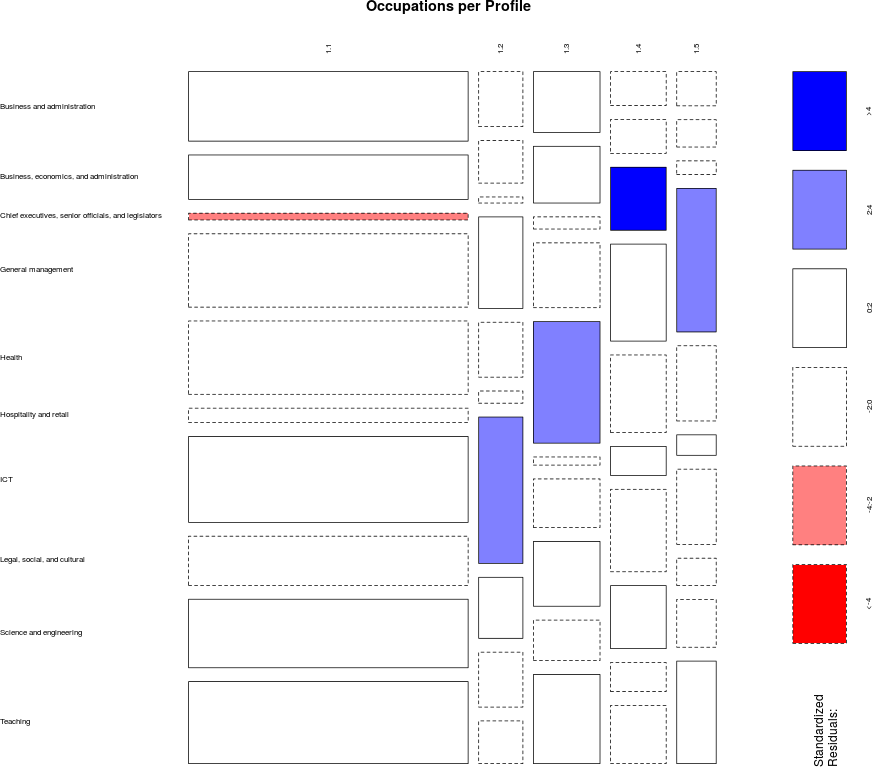
\includegraphics{/home/stlk/projects/appcentriccomp/reports/030_latent_profile_analysis_files/figure-latex/unnamed-chunk-11-1.png}
\caption{MosaicPlot - blue color indicates that occupation is prominent
more than expected, red - less than expected}
\end{figure}

\begin{verbatim}
## null device 
##           1
\end{verbatim}

\section{Statistical Testing Block}\label{statistical-testing-block}

Here I am constructing simple variables like number of:

\begin{itemize}
\tightlist
\item
  unique software used = n\_unique\_soft
\item
  unique software use per device\\
\item
  software used out of the top-10 popular items =
  n\_unique\_soft\_non\_pop
\item
  software use out of the top-10 popular per device =
  n\_unique\_soft\_per\_q\_non\_pop\footnote{I used camelCase versions
    of the variables later - latex does not get well with ``\_\_"
    symbols}.
\end{itemize}

I do not completely understand which theoretical constructs they do
represent yet, but found them useful in testing differences between
profiles later.

\subsection{Testing difference between reprogrammibility capabilities
across
Profiles}\label{testing-difference-between-reprogrammibility-capabilities-across-profiles}

In the current case when the LPA was accomplished considering difference
in the Q8\_v2\_ items it doesn't make much sense to compare them
statistically across profiles, but still might give some information
about profiles/

\begin{verbatim}
## 
##  Kruskal-Wallis rank sum test
## 
## data:  Q8_v2_1 by profile
## Kruskal-Wallis chi-squared = 340.15, df = 4, p-value < 2.2e-16
\end{verbatim}

\begin{verbatim}
## 
##  Kruskal-Wallis rank sum test
## 
## data:  Q8_v2_2 by profile
## Kruskal-Wallis chi-squared = 156.18, df = 4, p-value < 2.2e-16
\end{verbatim}

\begin{verbatim}
## 
##  Kruskal-Wallis rank sum test
## 
## data:  Q8_v2_3 by profile
## Kruskal-Wallis chi-squared = 362.54, df = 4, p-value < 2.2e-16
\end{verbatim}

\begin{verbatim}
## 
##  Kruskal-Wallis rank sum test
## 
## data:  Q8_v2_4 by profile
## Kruskal-Wallis chi-squared = 148.82, df = 4, p-value < 2.2e-16
\end{verbatim}

\subsection{Post hoc testing}\label{post-hoc-testing}

While we know, that there is a difference across profiles, we don't know
which profiles have differences (all of them?).

\begin{table}

\caption{\label{tab:unnamed-chunk-14}m3$Q8_v2_1 and m3$profile}
\centering
\begin{tabu} to \linewidth {>{\raggedright}X>{\raggedleft}X>{\raggedleft}X>{\raggedleft}X>{\raggedleft}X}
\hline
  & 1 & 2 & 3 & 4\\
\hline
2 & 1.000 & NA & NA & NA\\
\hline
3 & 0.000 & 0.000 & NA & NA\\
\hline
4 & 0.005 & 0.115 & 0 & NA\\
\hline
5 & 0.005 & 0.059 & 0 & 1\\
\hline
\end{tabu}
\end{table}

\begin{table}

\caption{\label{tab:unnamed-chunk-14}m3$Q8_v2_2 and m3$profile}
\centering
\begin{tabu} to \linewidth {>{\raggedright}X>{\raggedleft}X>{\raggedleft}X>{\raggedleft}X>{\raggedleft}X}
\hline
  & 1 & 2 & 3 & 4\\
\hline
2 & 0.000 & NA & NA & NA\\
\hline
3 & 0.000 & 0.000 & NA & NA\\
\hline
4 & 0.104 & 0.000 & 0 & NA\\
\hline
5 & 0.007 & 0.002 & 0 & 1\\
\hline
\end{tabu}
\end{table}

\begin{table}

\caption{\label{tab:unnamed-chunk-14}m3$Q8_v2_3 and m3$profile}
\centering
\begin{tabu} to \linewidth {>{\raggedright}X>{\raggedleft}X>{\raggedleft}X>{\raggedleft}X>{\raggedleft}X}
\hline
  & 1 & 2 & 3 & 4\\
\hline
2 & 0.00 & NA & NA & NA\\
\hline
3 & 0.00 & 0 & NA & NA\\
\hline
4 & 0.22 & 0 & 0 & NA\\
\hline
5 & 0.00 & 0 & 0 & 0\\
\hline
\end{tabu}
\end{table}

\begin{table}

\caption{\label{tab:unnamed-chunk-14}m3$Q8_v2_4 and m3$profile}
\centering
\begin{tabu} to \linewidth {>{\raggedright}X>{\raggedleft}X>{\raggedleft}X>{\raggedleft}X>{\raggedleft}X}
\hline
  & 1 & 2 & 3 & 4\\
\hline
2 & 0.000 & NA & NA & NA\\
\hline
3 & 0.000 & 0 & NA & NA\\
\hline
4 & 0.035 & 0 & 0 & NA\\
\hline
5 & 0.000 & 1 & 0 & 0.001\\
\hline
\end{tabu}
\end{table}

\subsubsection{Plot the differences across
profiles}\label{plot-the-differences-across-profiles}

TODO: put significance levels

\begin{figure}[htbp]
\centering
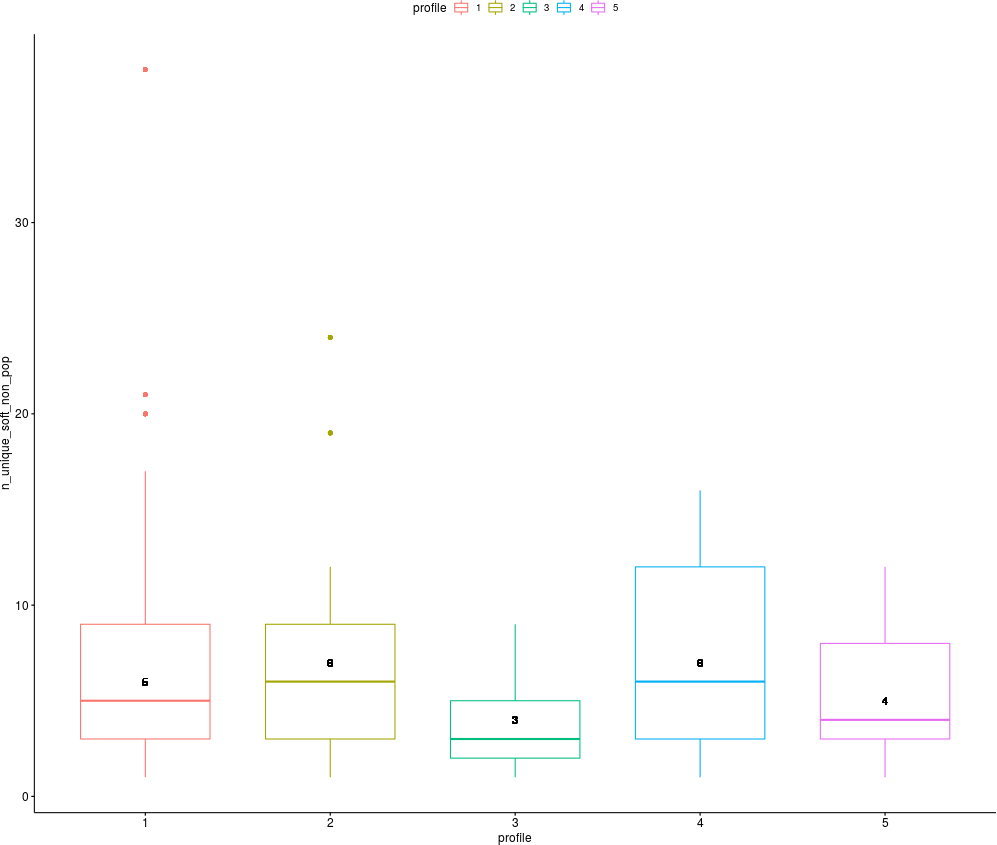
\includegraphics{/home/stlk/projects/appcentriccomp/reports/030_latent_profile_analysis_files/figure-latex/unnamed-chunk-15-1.png}
\caption{Difference in Soft Used out Of Top-10 Across Profiles}
\end{figure}

\subsection{Turning Back}\label{turning-back}

Let's return to the variables we've constructed earlier - since they
were not included into the LPA it makes much more sense to include them
in profile difference hypotheses testing.

We use bonferroni p-value adjustment since we simultaneously testing
several hypotheses. P-values smaller than .05 indicate difference in
groups given variable. I have not provided interpretation yet, since LPA
and grouping might and probably will be changed.

\begin{table}

\caption{\label{tab:unnamed-chunk-16}tmp$nUniqueSoftPerqNonPop and tmp$profile}
\centering
\begin{tabu} to \linewidth {>{\raggedright}X>{\raggedleft}X>{\raggedleft}X>{\raggedleft}X>{\raggedleft}X}
\hline
  & 1 & 2 & 3 & 4\\
\hline
2 & 1.000 & NA & NA & NA\\
\hline
3 & 0.000 & 0.000 & NA & NA\\
\hline
4 & 0.327 & 0.632 & 0.000 & NA\\
\hline
5 & 0.236 & 0.308 & 0.305 & 1\\
\hline
\end{tabu}
\end{table}

\begin{table}

\caption{\label{tab:unnamed-chunk-16}tmp$nUniqueSoftNonPop and tmp$profile}
\centering
\begin{tabu} to \linewidth {>{\raggedright}X>{\raggedleft}X>{\raggedleft}X>{\raggedleft}X>{\raggedleft}X}
\hline
  & 1 & 2 & 3 & 4\\
\hline
2 & 1.000 & NA & NA & NA\\
\hline
3 & 0.000 & 0.000 & NA & NA\\
\hline
4 & 1.000 & 1.000 & 0 & NA\\
\hline
5 & 0.079 & 0.062 & 0 & 0.157\\
\hline
\end{tabu}
\end{table}

\begin{table}

\caption{\label{tab:unnamed-chunk-16}tmp1$nUniqueSoft and tmp$profile}
\centering
\begin{tabu} to \linewidth {>{\raggedright}X>{\raggedleft}X>{\raggedleft}X>{\raggedleft}X>{\raggedleft}X}
\hline
  & 1 & 2 & 3 & 4\\
\hline
2 & 1.000 & NA & NA & NA\\
\hline
3 & 1.000 & 1.000 & NA & NA\\
\hline
4 & 0.427 & 0.053 & 0.153 & NA\\
\hline
5 & 0.007 & 0.002 & 0.005 & 0.672\\
\hline
\end{tabu}
\end{table}

\end{document}
